%
% Modified by Megan Patnott
% Last Change: Jan 18, 2013
%
%%%%%%%%%%%%%%%%%%%%%%%%%%%%%%%%%%%%%%%%%%%%%%%%%%%%%%%%%%%%%%%%%%%%%%%%
%
% Modified by Sameer Vijay
% Last Change: Tue Jul 26 2005 13:00 CEST
%
%%%%%%%%%%%%%%%%%%%%%%%%%%%%%%%%%%%%%%%%%%%%%%%%%%%%%%%%%%%%%%%%%%%%%%%%
%
% Sample Notre Dame Thesis/Dissertation
% Using Donald Peterson's ndthesis classfile
%
% Written by Jeff Squyres and Don Peterson
%
% Provided by the Information Technology Committee of
%   the Graduate Student Union
%   http://www.gsu.nd.edu/
%
% Nothing in this document is serious except the format.  :-)
%
% If you have any suggestions, comments, questions, please send e-mail
% to: ndthesis@gsu.nd.edu
%
%%%%%%%%%%%%%%%%%%%%%%%%%%%%%%%%%%%%%%%%%%%%%%%%%%%%%%%%%%%%%%%%%%%%%%%%


%
% Chapter 3
%

\chapter{EXPERIMENTAL APPARATUS}

\section{The Large Hadron Collider}
The most powerful machine of its kind, the Large Hadron
Collider (LHC) accelerates and collides particles
at high center-of-mass energies producing rare
particles and interactions that would be otherwise unobservable
in the laboratory, making it the best tool available for studying \tth
processes. The LHC is a circular particle accelerator/collider. Measuring 27 km
in circumference, it collides beams of protons in head-on collisions       
at a center-of-mass energy of 13 TeV.

Originally conceived in the early 1980s and approved in 1994, the LHC was designed to replace the then-operating
Large Electron Positron Collider (LEP), re-using the same underground tunnel. Located just outside Geneva, Switzerland, at the Center for European Nuclear Research (CERN),
the LHC stretches across the border into France. There are four detector experiments positioned around the LHC-ALICE, ATLAS, CMS, and LHCb. The two general purpose,
functionally-equivalent detectors are ATLAS and CMS, while ALICE studies heavy ion collisions, and LHCb studies flavor physics. 
The motivation for having two equivalent detectors is to provide cross checks on results, as each result is produced with separate analysis teams, studying separate collsions
recorded with a separate detector. Each detector is centered on an interaction point, where the beams are steered into each other to produce collisions. 
The LHC itself is technically the final element in a series of accelerators
that bring beams from rest to succesively higher energies. This system of
of accelerators, referred to as the LHC Accelerator Complex is depicted below in
Figure~\ref{fig:lhc_complex}.

The acceleration is accomplished with radio frequency
(RF) cavities. RF cavities are a linear series of cylindrical conductors,
which sustain a resonant electromagnetic field produced by a generator. As 
charged particles pass through the cavities, they experience a force
(acceleration) from the resonant alternating field in each cavity. This acceleration process begins with Hydrogen gas in the linear accelerator
(LINAC 2). The Hydrogen atoms in the gas are stripped of electrons
in an applied electric field, leaving only protons, which are then accelerated
along the linear beam pipe with RF cavities to an energy of 50 MeV. After the LINAC, the beams of protons enter the Proton Synchrontron Booster rings where
they are accelerated to 1.4 GeV, before reaching the Proton
Synchrotron (PS). The circular PS, measuring more than 600 m
in circumference, accelerates the beams to 25 GeV before injection into the
larger, Super Proton Synchrotron (SPS). The SPS at over 7 km around, provides the final
acceleration before the beams reach the LHC at an energy 450 GeV. The SPS injects the beams into
the LHC in opposite directions. After the beams are fully injected, the LHC ramps the beam energy to 6.5 TeV per beam, providing 13 TeV center-of-mass proton collisions.

The beam pipes of the entire accelerator complex are kept at an ultra high vaccuum
to avoid detrimental beam interactions before the collisions. Since the beams are made up of protons which have electric charge,
they can be focused and steered around the LHC with 392 quadrupole and 1232 dipole superconducting magnets.
To accomplish this, the magnets produce a field of over 8 Tesla. This is possible thanks to the
superconducting niobium-titanium coils which are cooled with liquid nitrogren and superfluid helium-4. These
magnets operate at 1.9 K allowing them to carry a current of over 11000 amperes. In addition to
the LHC, superconducting magnets are used throughout the accelerator complex.

Inside the LHC, the beams travel in opposite directions in separate but adjacent pipes inside of the superconducting magnets.
As a result of the RF cavity acceleration, the beams are comprised of individual 'bunches' of protons.
There are over 2800 bunches in each beam, with each bunch spaced 25 ns apart. This spacing is choosen to
produce as many bunch crossings as possible, without overloading
the detector instrumentation and data acquisition. There are approximately $10^{11}$ protons in each bunch, but due to the small cross section of the protons,
only approximately 20 collisions occur in each bunch crossing. The beams travel around the LHC over 11,246 times per second, over 99.99$\%$ the speed of light. 
This translates to around 600 million collisions per second.

The center-of-mass energy and time-spacing between proton bunches in the LHC are critical to studying interesting
and rare physics processes. A sufficient center-of-mass collision energy is needed to produce new, heavy particles.
With the current center-of-mass collision energy of 13 TeV, any particle with mass less than or equal to this, is 
within reach of the LHC. Because many interesting physics processes are exceedingly rare (small cross section), many collisions
are needed. The quantity used to describe the number of collisions occuring is called Luminosity.
Described in equation~\ref{eqn:lumi_inst} below, instantaneous luminosity represents the number of collisions (events) occuring per unit time.

\begin{equation}
\label{eqn:lumi_inst}
 \mathcal{L}_{inst} = \frac{N_{b}^{2}n_{b}f_{\textnormal{rev}}\gamma}{4\pi \epsilon_{n} \beta^{*}}F
\end{equation}

Where $N_{b}$ is the number of protons per bunch, $n_{b}$ is the total number of bunches, $f_{\textnormal{rev}}$ is the number of beam revolutions around the LHC per
second, $\gamma$ is a relativistic factor, $\epsilon_{n}$ is factor related to beam emittance, $\beta^{*}$ is the beta function representing the beam cross section, and
$F$ describes the factor related to the crossing angle of the beams. Because not every collision can be recorded, knowing the total number of collisions is critically important
to every analysis at an LHC collider experiment. From the instantaneous luminosity, the total number of collisions in time interval $t$ can be calculated by integrating over time
in equation~\ref{eqn:num_coll} below. 

\begin{equation}
\label{eqn:num_coll}
N_{pp} = \int \sigma_{pp}\mathcal{L}_{inst}dt 
\end{equation}


\begin{figure}[hbtp]
 \begin{center}
   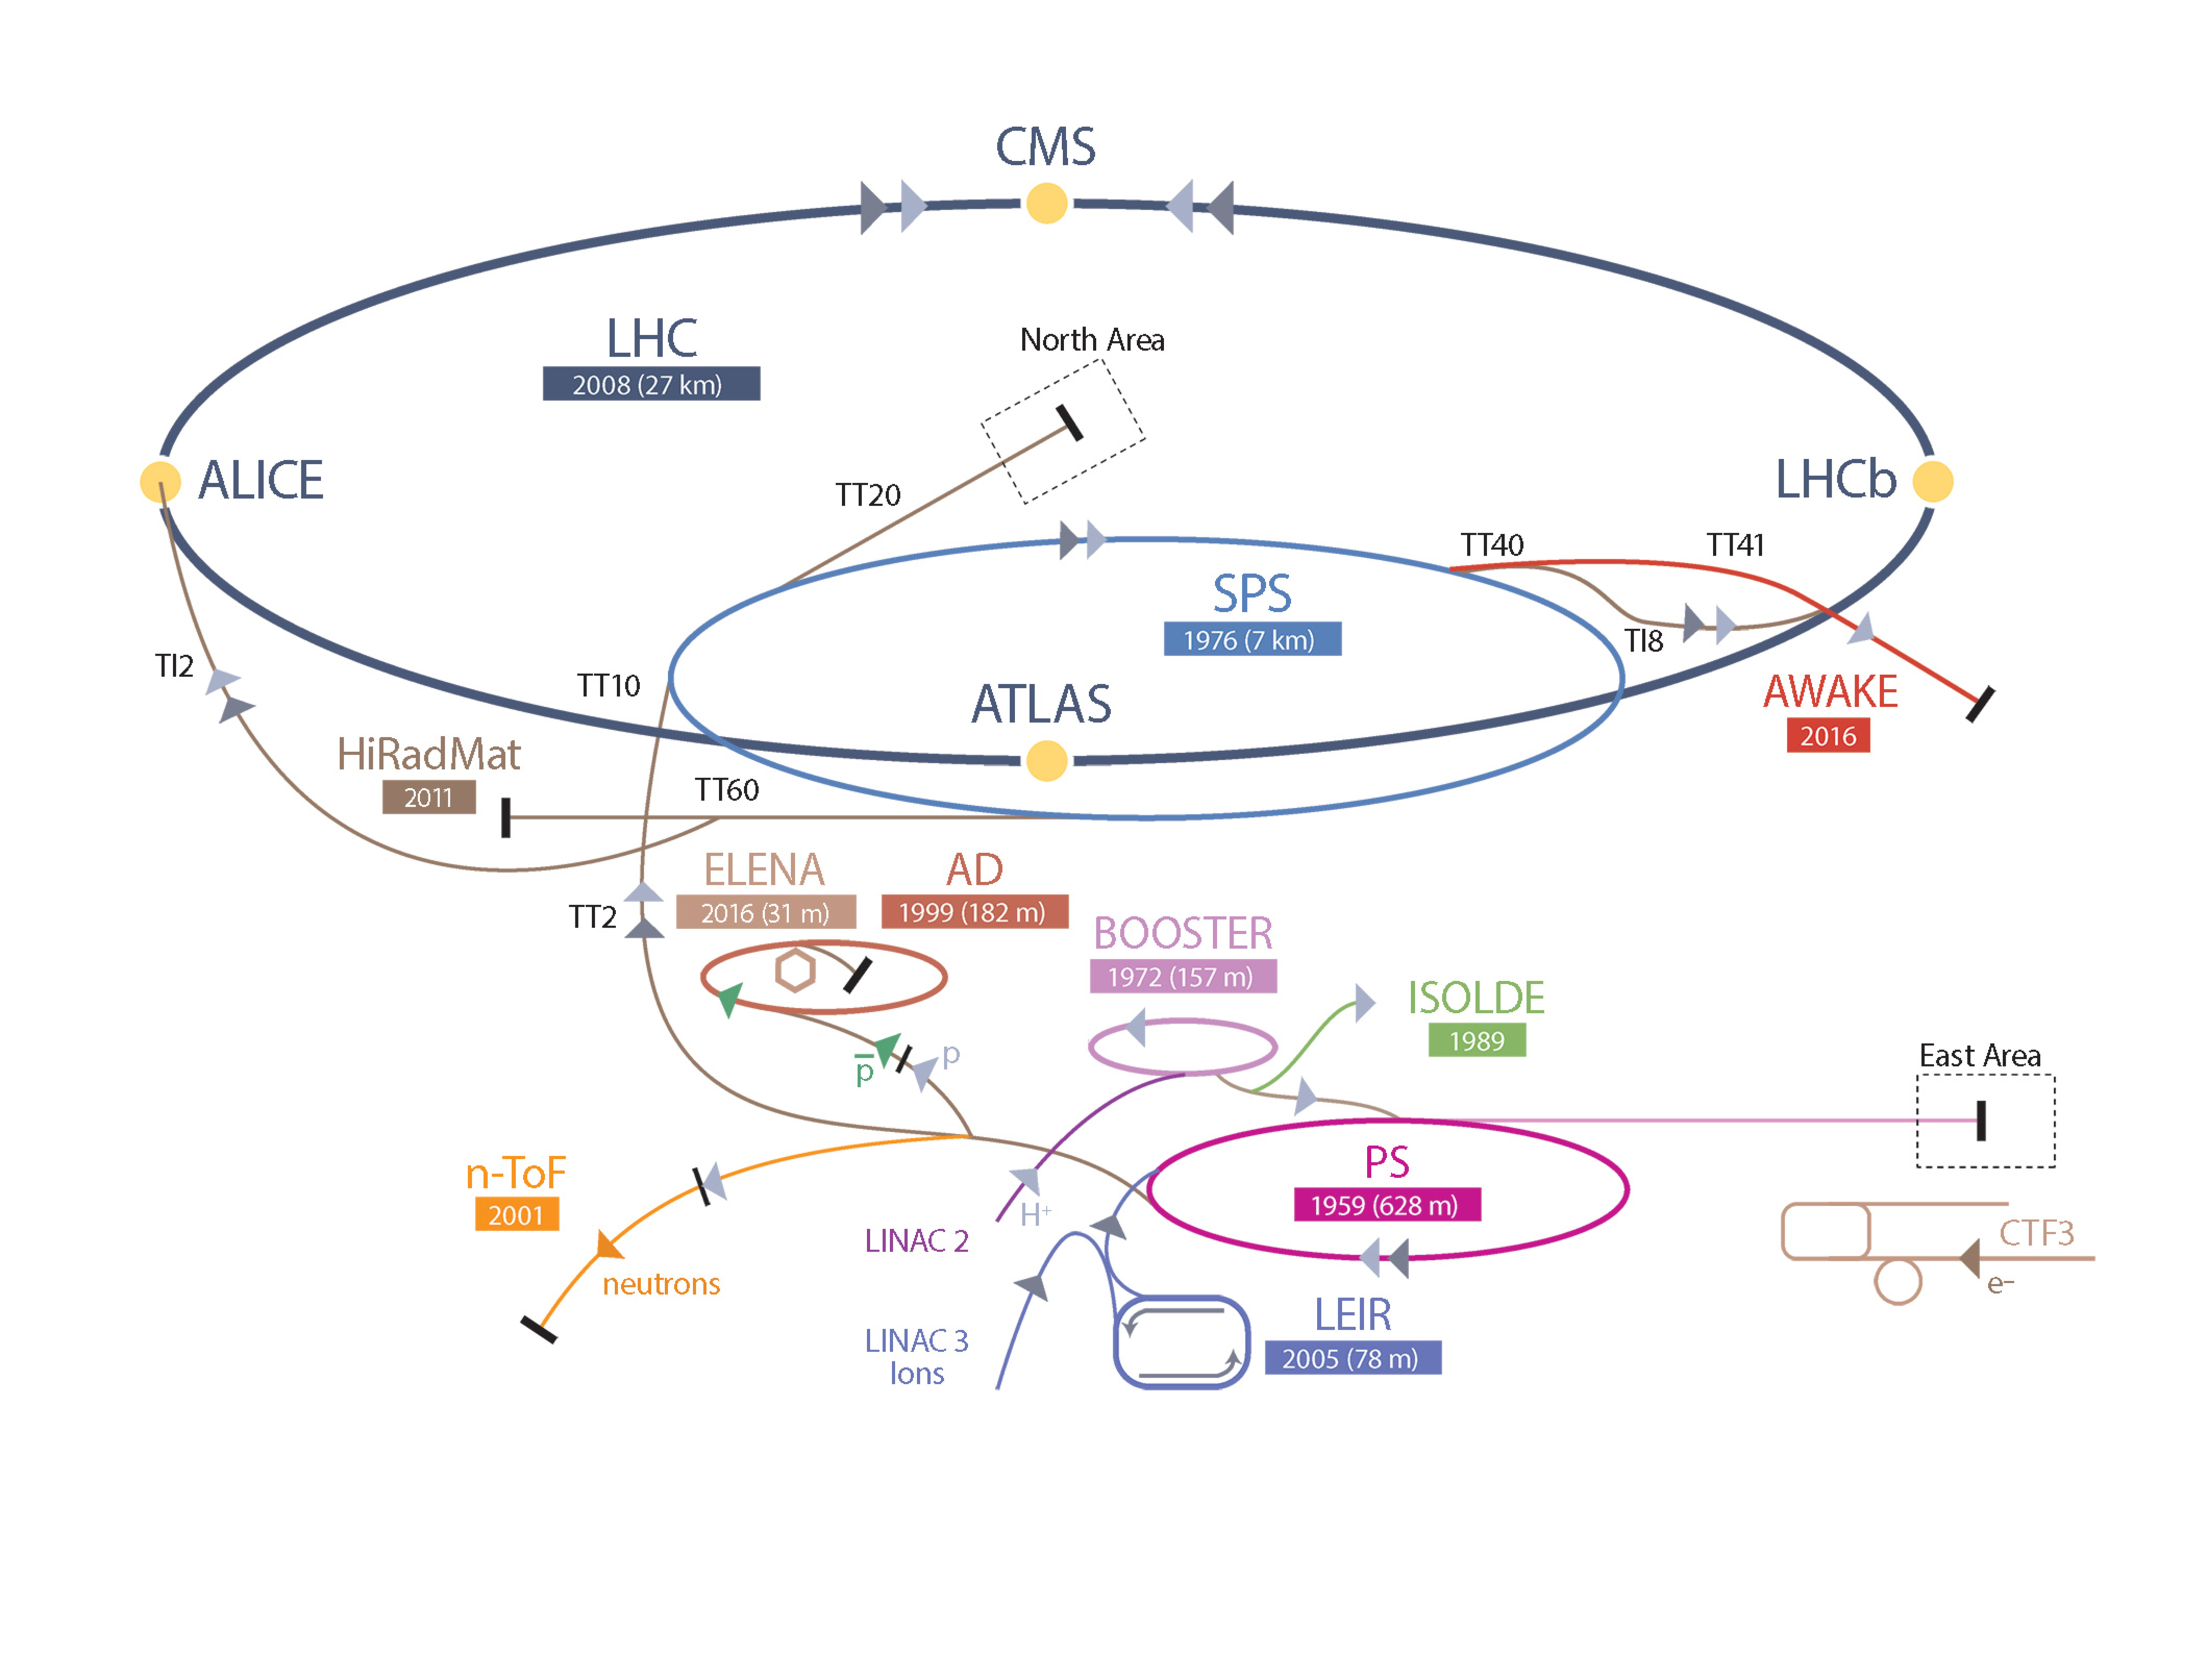
\includegraphics[width=0.9\textwidth]{lhc_complex.pdf}
   \caption[text in square brackets]{An overview of the LHC accelerator complex.}
   \label{fig:lhc_complex}
 \end{center}
\end{figure}


\section{The Compact Muon Solenoid (CMS) Detector}
The Compact Muon Solenoid (CMS) detector is a multi purpose particle detector designed to record and identify particles produced in collisions at the LHC, sitting 100 m underneath
the town of Cessy, France. CMS is comprised of layers of subdetectors which are connected to the trigger system and the data acquisition system.
The various subdetectors record information about the collision, while the trigger system and
data acquisition systems record and save the collisions. The acronym CMS comes from being more compact than its sister detector ATLAS, at 15 m in diameter and
over 21 m long. The name muon is because muons are the particles it detects with the greatest efficiency. The solenoid part of the name is due to the largest magnet of its kind
around which the detector is built. CMS is cylindrical in shape, as pictured in Figure~\ref{fig:cms_overview}. The various subdetectors and components are described in more
below. 

\begin{figure}[hbtp]
 \begin{center}
   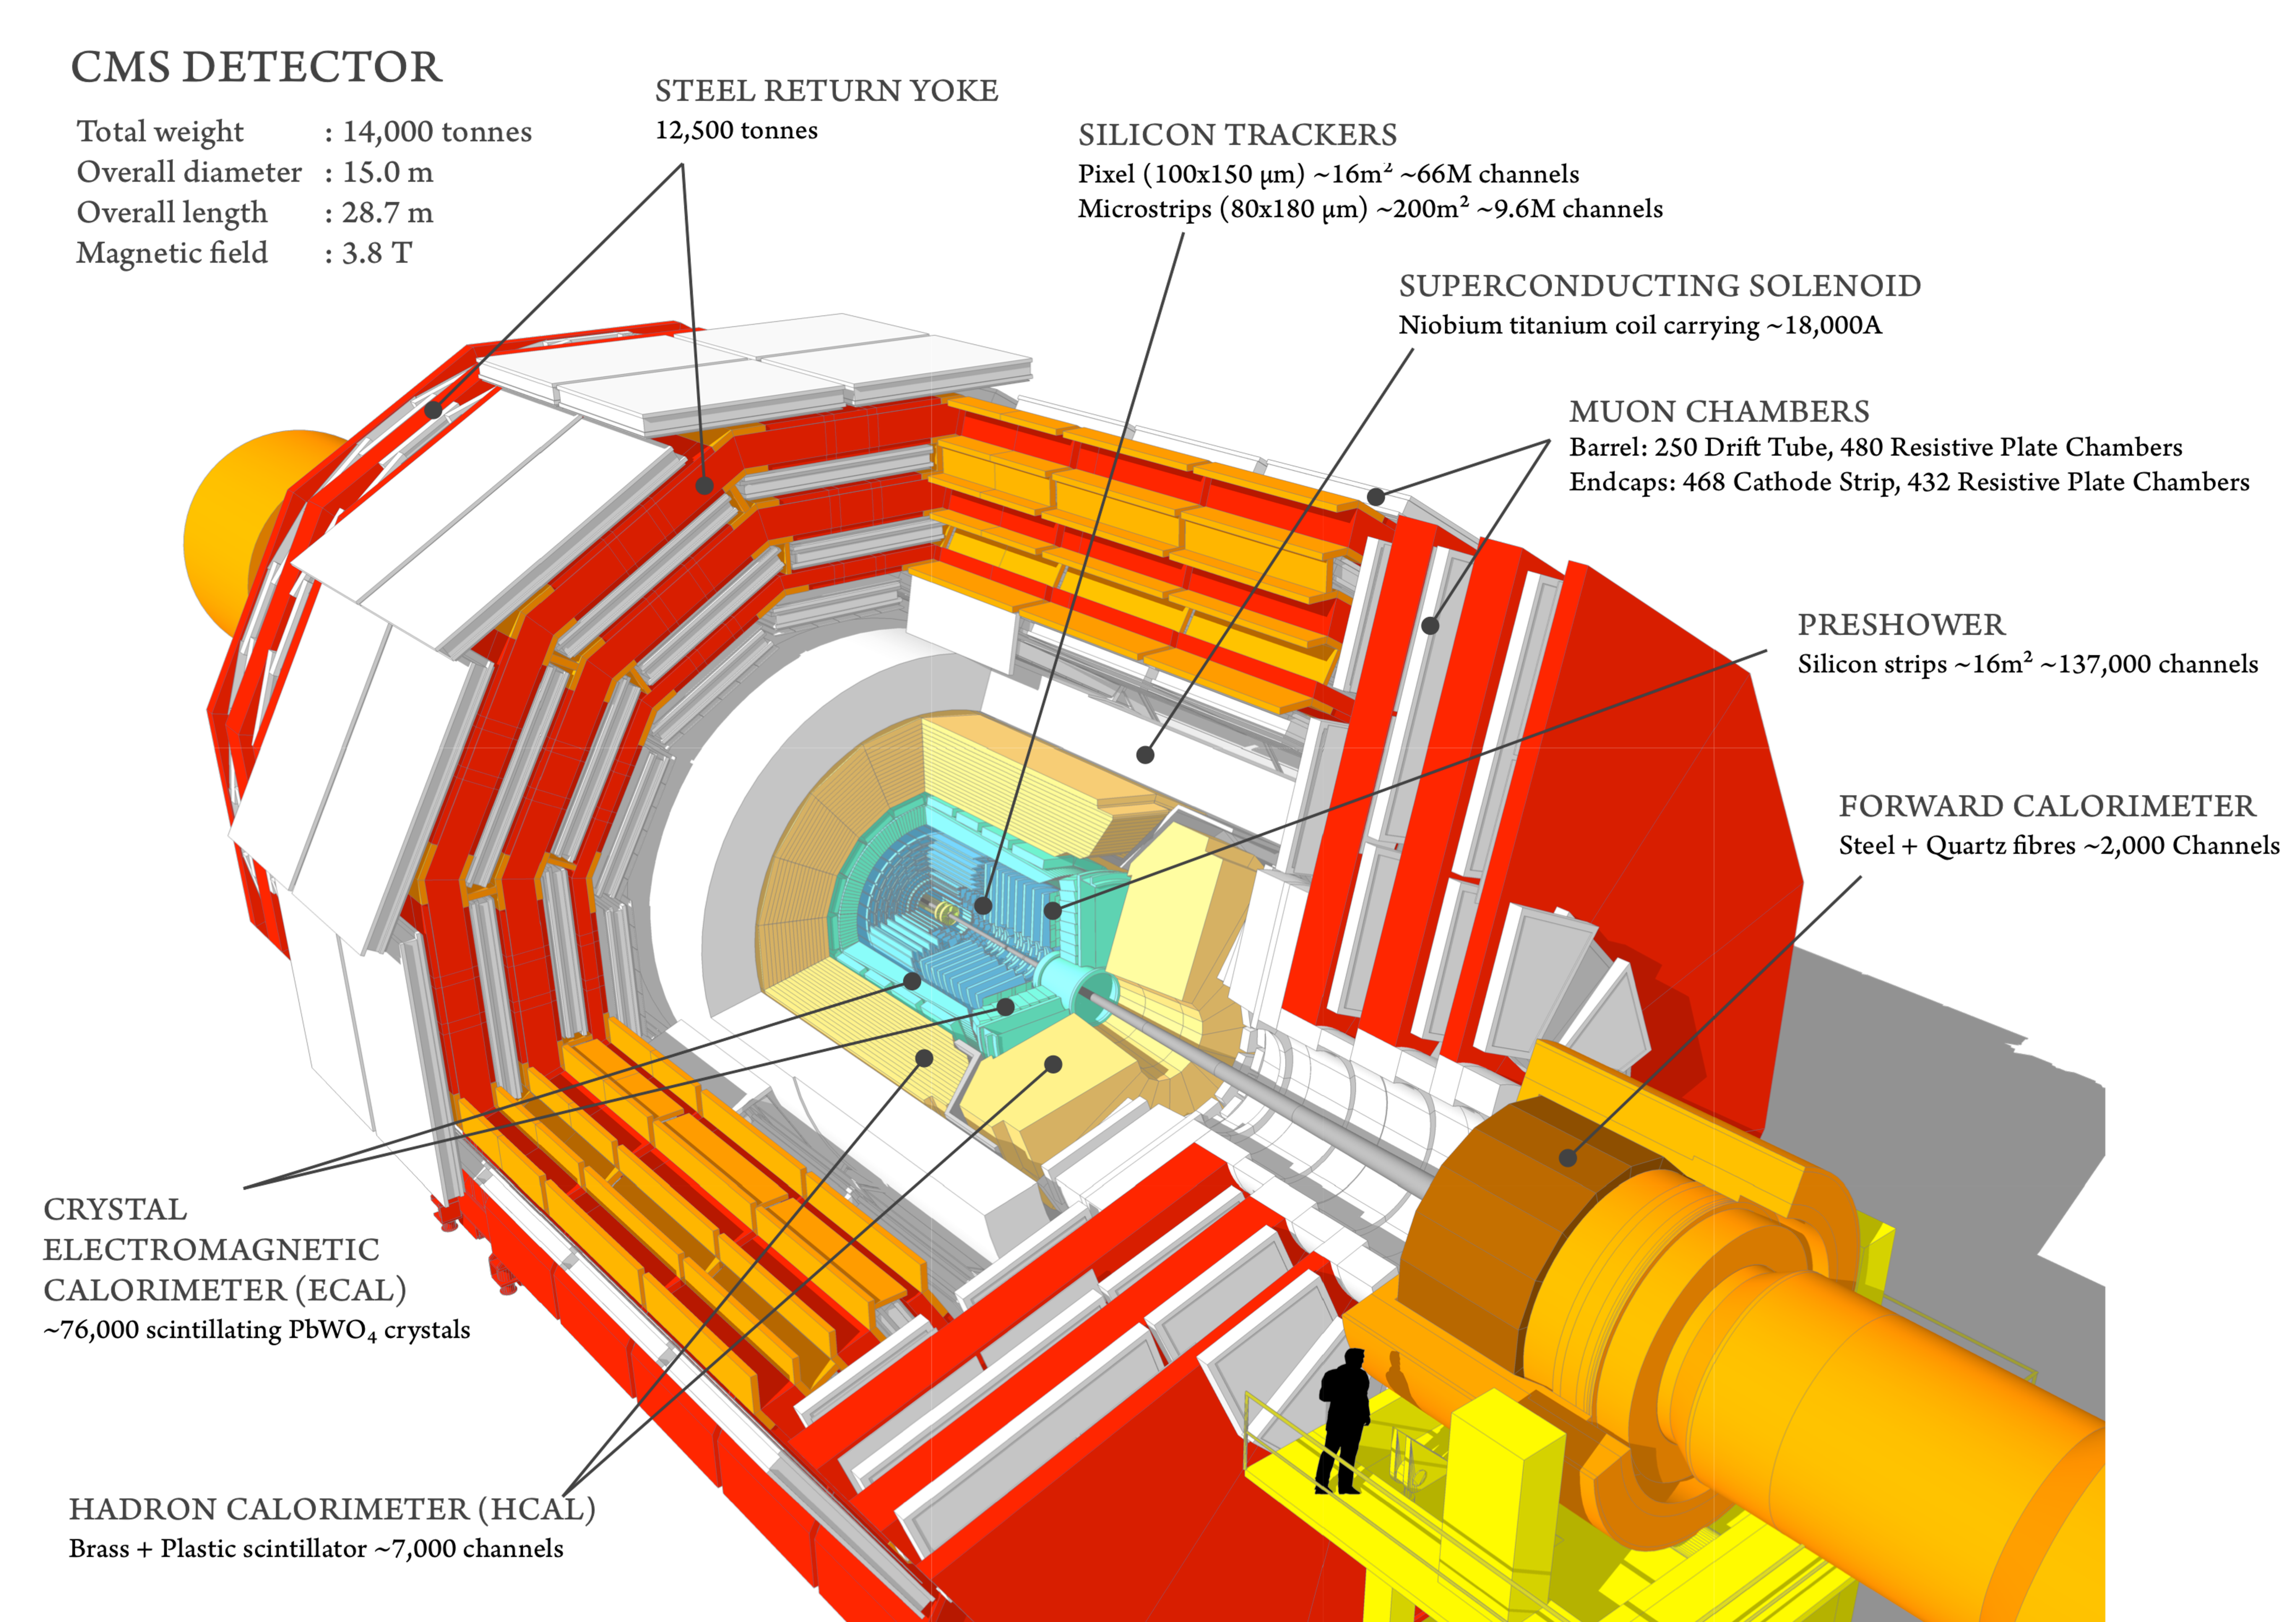
\includegraphics[width=0.9\textwidth]{cms_overview.pdf}
   \caption[text in square brackets]{A qualitative overview of the CMS detector.}
   \label{fig:cms_overview}
 \end{center}
\end{figure}

\subsection{Coordinate System}
Due to the geometry of the collisions produced inside CMS, a special coordinate system is used for simplicity. With the origin at the interaction point,
the y-axis in the verical direction, the z-axis parallel to/along the beam direction, and the x-axis in the horizontal direction, perpendicular to both the y
and z axes. In the transverse x-y plane, the angle formed with respect to the x-axis is $\phi$. In the y-z plane, the angle formed with respect to the z-axis
is $\theta$. The number of particles traveling through a given area, known as flux, increases towards the beam line, due to many more glancing collisons ocurring
than head-on collisions. The particles from the collisions are moving relativistically. Because of this, a special coordinate $\eta = -\ln\tan(\theta/2)$ 
is used to describe the angular position with respect to the z-axis, known as $pseudorapidity$. The head-on inelastic pp collisions have only momentum in the 
z-direction, thus measuring energy and momentum quantities in the transverse plane is important in analyzing and reconstructing collision events due to momentum
conservation.  

\subsection{Tracker}
\subsubsection{Pixel Detector}
The innermost piece of CMS is the tracking system, specifically the pixel detector. The pixel detector is comprised of 65 million silicon pixels, allowing it to record
precise trajectories of the charged particles resulting from collisions. Precise tracking information is critical to differentiating nearby particles, and identifying
exactly where an interesting collision took place. 

The pixel detector, about the size of a shoe box, contains 3 layers at 4 cm, 7 cm, and 11 cm from the beam.
The silicon material in the tracker is choosen specifically to disturb the particles as little as possible, while still providing accurate particle track reconstruction.
Additionally, the material is resistant to radiation, as it is only a few centimeters from the interaction point. Each pixel measurses 100 $\mu$m by 150 $\mu$m. 

As the particles travel through successive layers of silicon pixels, they leave points of impact on each pixel, known as hits.
The hits are measured with a precision of 10 $\mu$m, and the particle trajectory or track is reconstructed from collections of hits. 
As a particle travels through a pixel, it releases electrons from the silicon atoms, creating electron-hole pairs.
A voltage is applied to the pixel, attracting the free electrons and creating a small current, which is measured and translated to a hit. Small readout electronics
are attached to the back of each pixel to send the hit information to the data acquisition system, so the hit patterns can be reconstructed into particle tracks later.   

\begin{figure}[hbtp]
 \begin{center}
   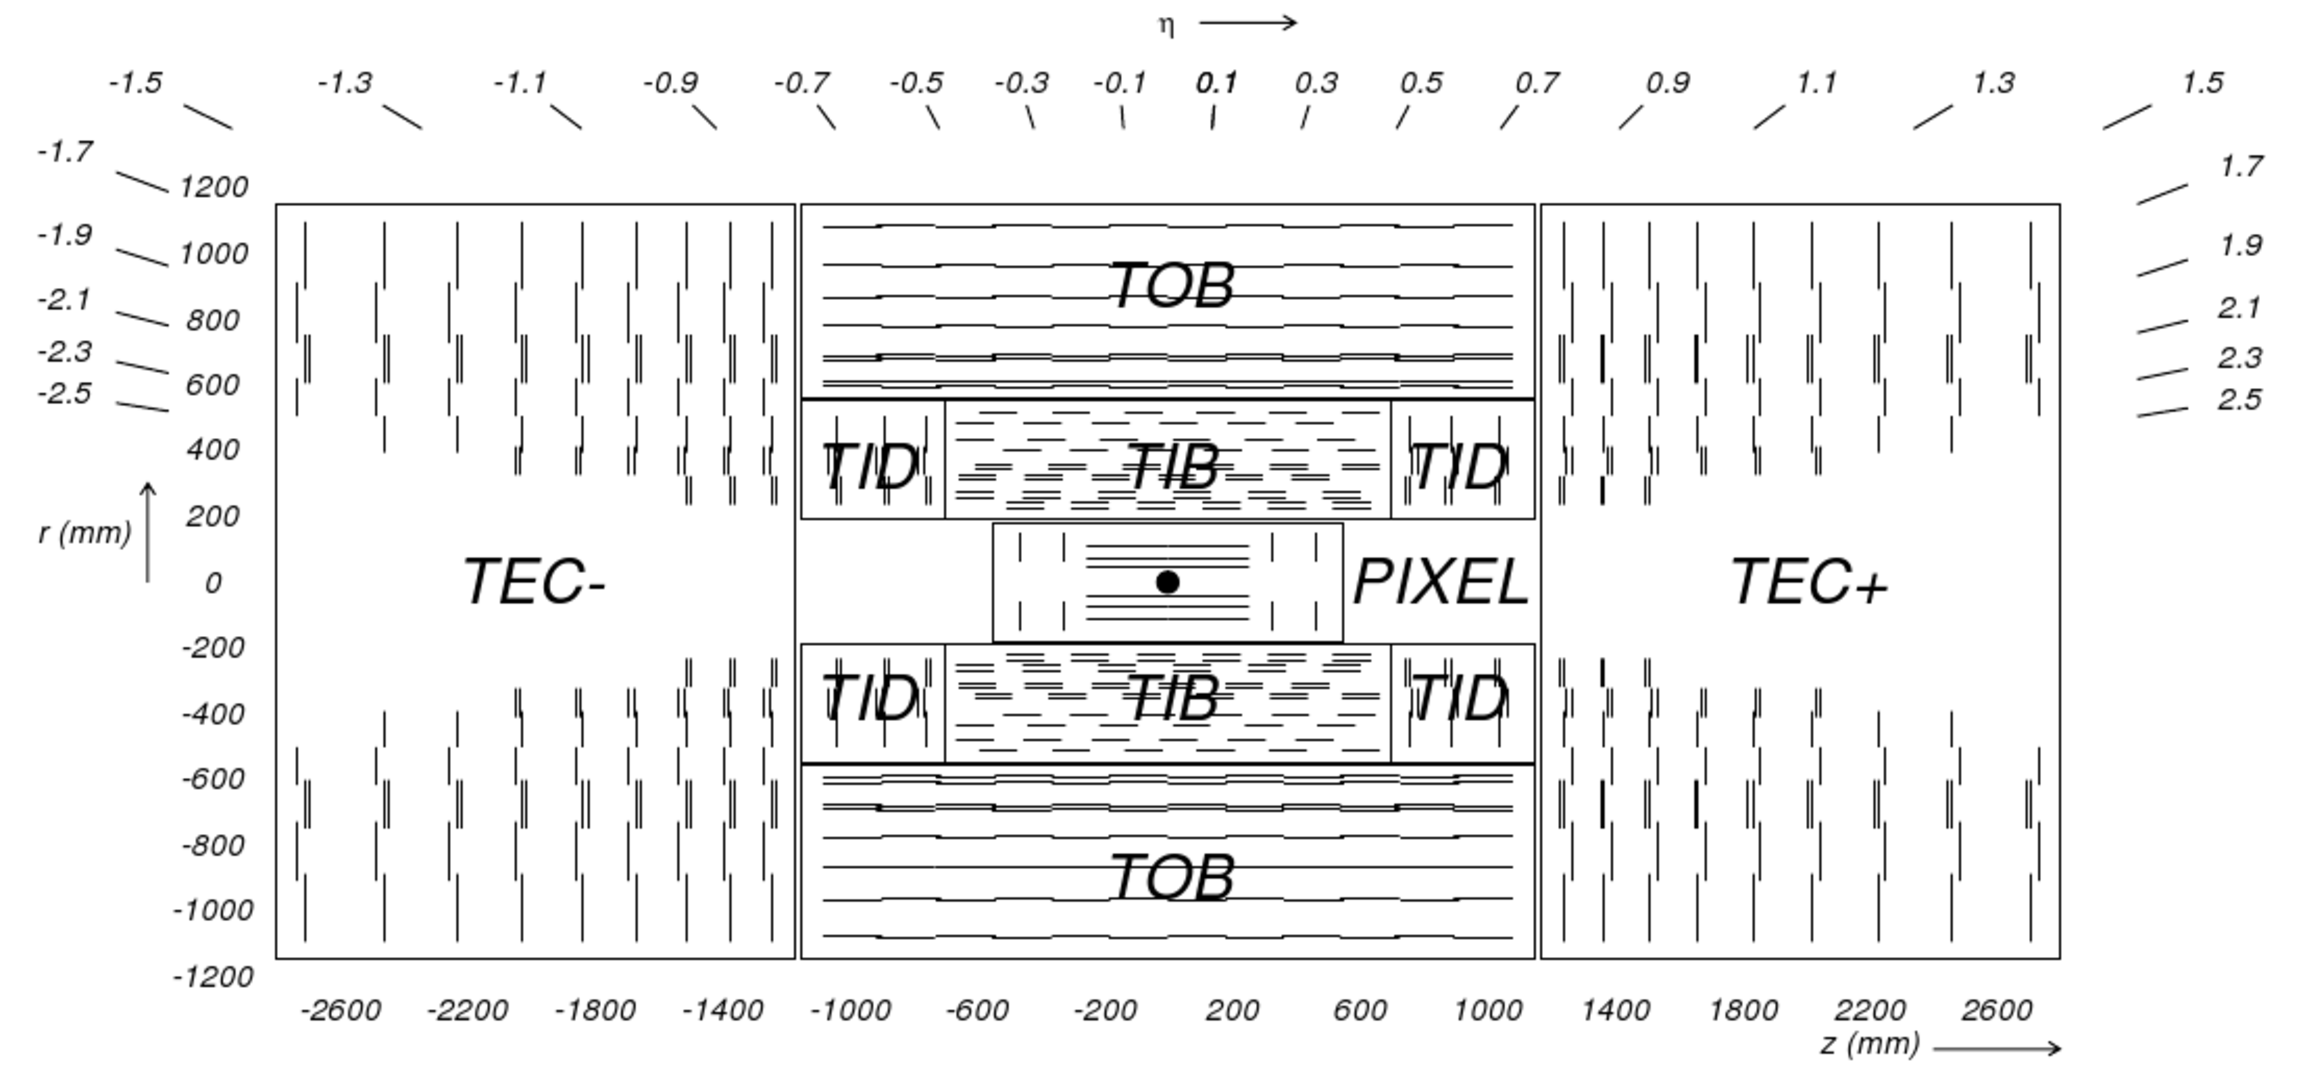
\includegraphics[width=0.6\textwidth]{tracker_yz.pdf}
   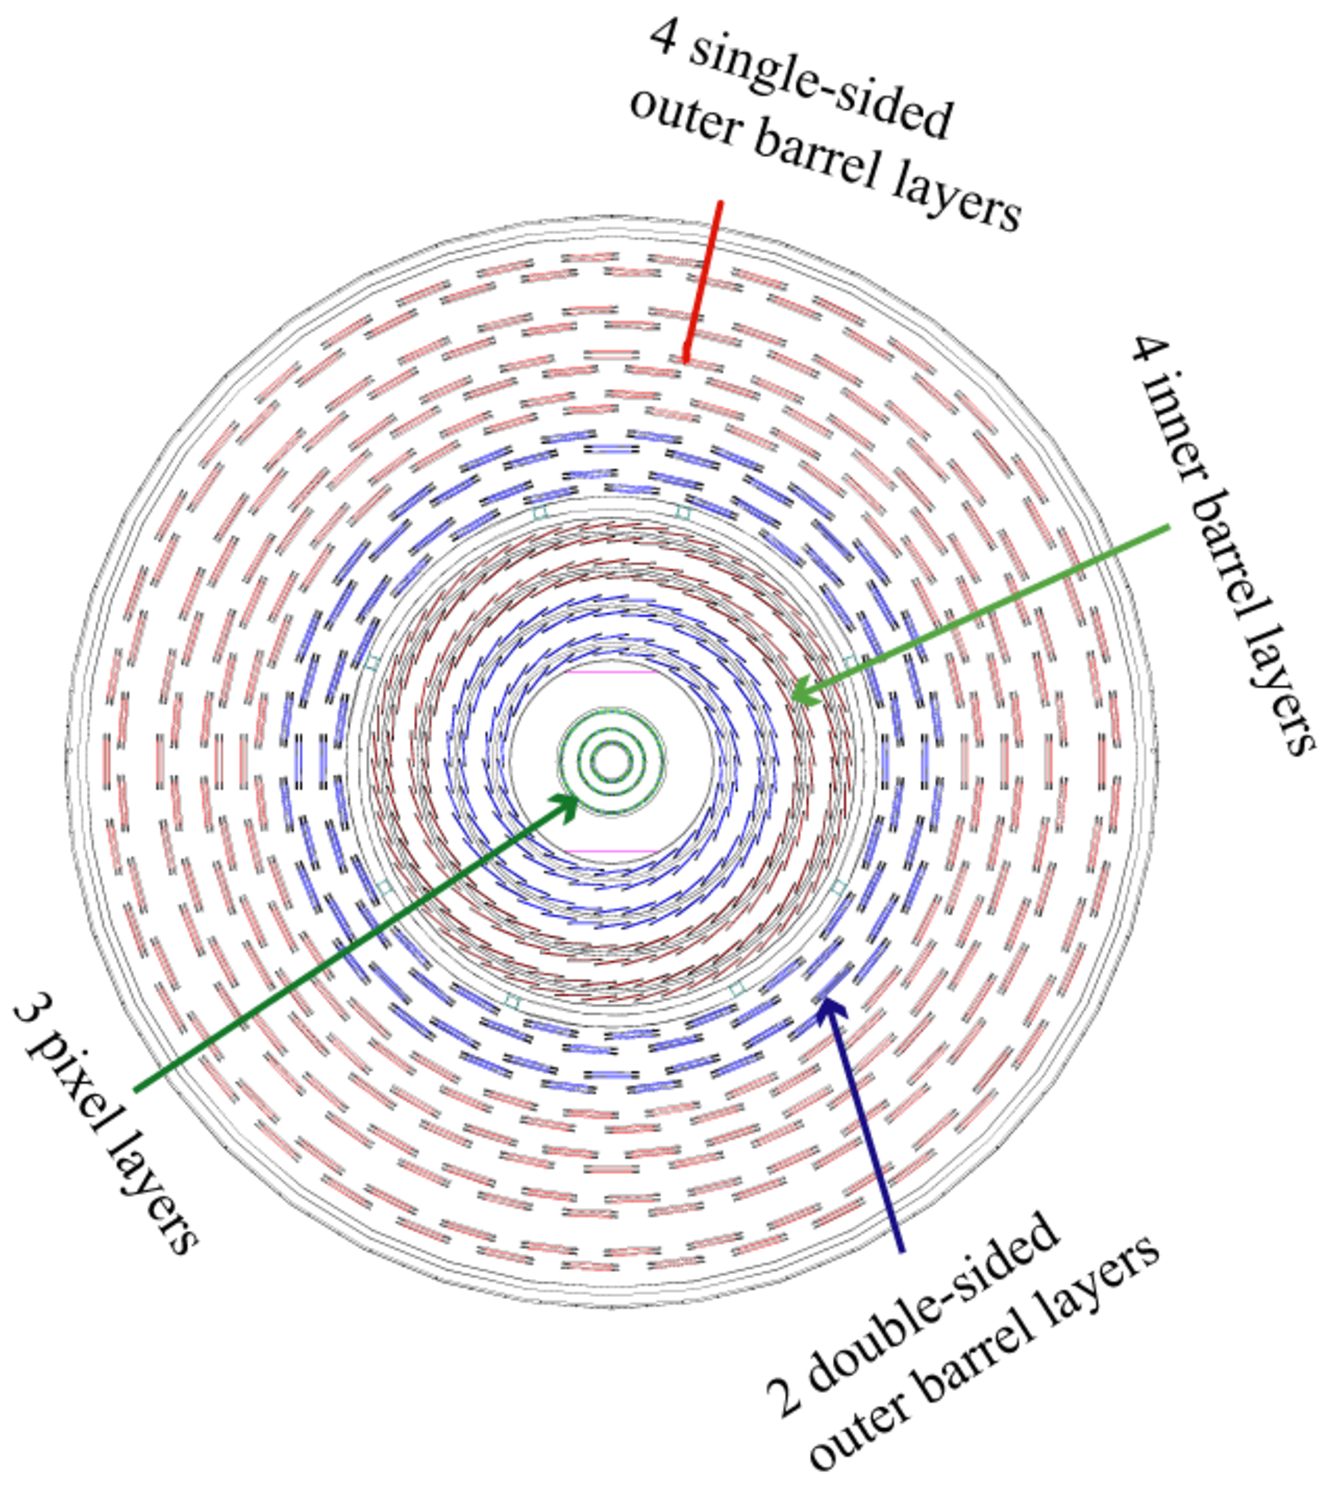
\includegraphics[width=0.25\textwidth]{tracker_transverse_layers.pdf}
   \caption[text in square brackets]{The CMS silicon tracking system including both the pixel and strip detectors in y-z plane (left), and tranverse x-y plane (right).}
   \label{fig:cms_tracker}
 \end{center}
\end{figure}

\subsubsection{Strip Detector}
Outside the pixel detector is the silicon strip detector. Here, silicon strips are favored over pixels as they are less costly, and the resolution provided by the pixels
is not necessary at greater distances from the interaction point, allowing for larger and fewer silicon modules. 

The silicon strip detector consists of about 10 million strips in 10 layers, extending to 130 cm from the beam. 
The strip detector is comprised of 4 distinct sections of silicon strips, depicted in
Figure~\ref{fig:cms_tracker}. The outer most sections are the tracker outer barrel (TOB) and tracker end cap (TEC+,-) sections. Between the TOB and the pixels, sits the tracker
inner barrel (TIB) section, and the tracker inner endcaps (TID+,-). The silicon strips in each section are different, specifically suited to that section.
Each silicon strip measures between 10-25 $\mu$m by 180 $\mu$m, depending on the section. The total detector area of the tracking system (pixels+strips) sums to more than
a tennis court of silicon. Precise tracking information is essential to measuring particle momenta and identifying particles in a strong magnetic field.

\subsection{ECAL}

The Electromagnetic Calorimeter (ECAL) measures the energy of particles that interact via the electromagnetic force. The ECAL is situated immediately outside tracker
and is made of up thousands of lead tungstate ($PbWO_{4}$) crystals in three sections. The ECAL provides good energy resolution and fast readouts,
which make it ideal for recording the frequent events produced by the LHC. 

The ECAL is made up of three sections; the barrel, endcaps, and preshower, depicted in Figure~\ref{fig:cms_ecal}. The barrel section is cylindrical and covers the full $\phi$
range, and extends between $|\eta| < 1.479$ in y-z. The barrel consists of 61200 crystals, each measuring approximately 2.2 cm x 2.2cm x 23 cm. The length of each barrel
crystal translates to approximately 26 radiation lengths. The two endcaps sit on each end of the barrel, extending between $1.479 < |\eta|< 3.0$, 315 cm on either side of
the interaction point. There 14648 identical crystals in the endcaps, each measuring 3 cm x 3 cm x 22 cm. Like the crystals in the barrel, these crystals have a small taper
with the smaller face pointing towards the interaction point. The preshower disc sits on the ends of the barrel and in front of the endcaps. The preshower measures 2.5 m in
circumference and is 20 cm thick. The ECAL preshower consists of two layers
of lead, followed by silicon sensors measuring 2mm x 2mm. The preshower allows ECAL to resolve nearby photon pairs, and discriminate against those coming from in-flight decays
of neutral pions. The scintillation light from each crystal is detected by an Avalanche Photo Diode (APD) in the barrel, and an Vaccuum Photo Triode (VPT) in the endcap.
These readouts convert the scintillation light to a voltage pulse that is passed futher downstream to the trigger and DAQ. 

After particles pass through the silicon tracking system, they enter ECAL. The ECAL measures the energy of the electrons and photons produced in the LHC collisions.
The choice of the lead tungstate material is motivated by needing to stop the particles, and also scintillate light effectively to allow an accurate energy readout and measurement
The stopping action is accomplished with the lead, while the scintillation is accomplished with
the crystalline oxygen. These combined properties produce photons (light) in proportion to the amount of energy deposited by the stopped particles.



\begin{figure}[hbtp]
 \begin{center}
   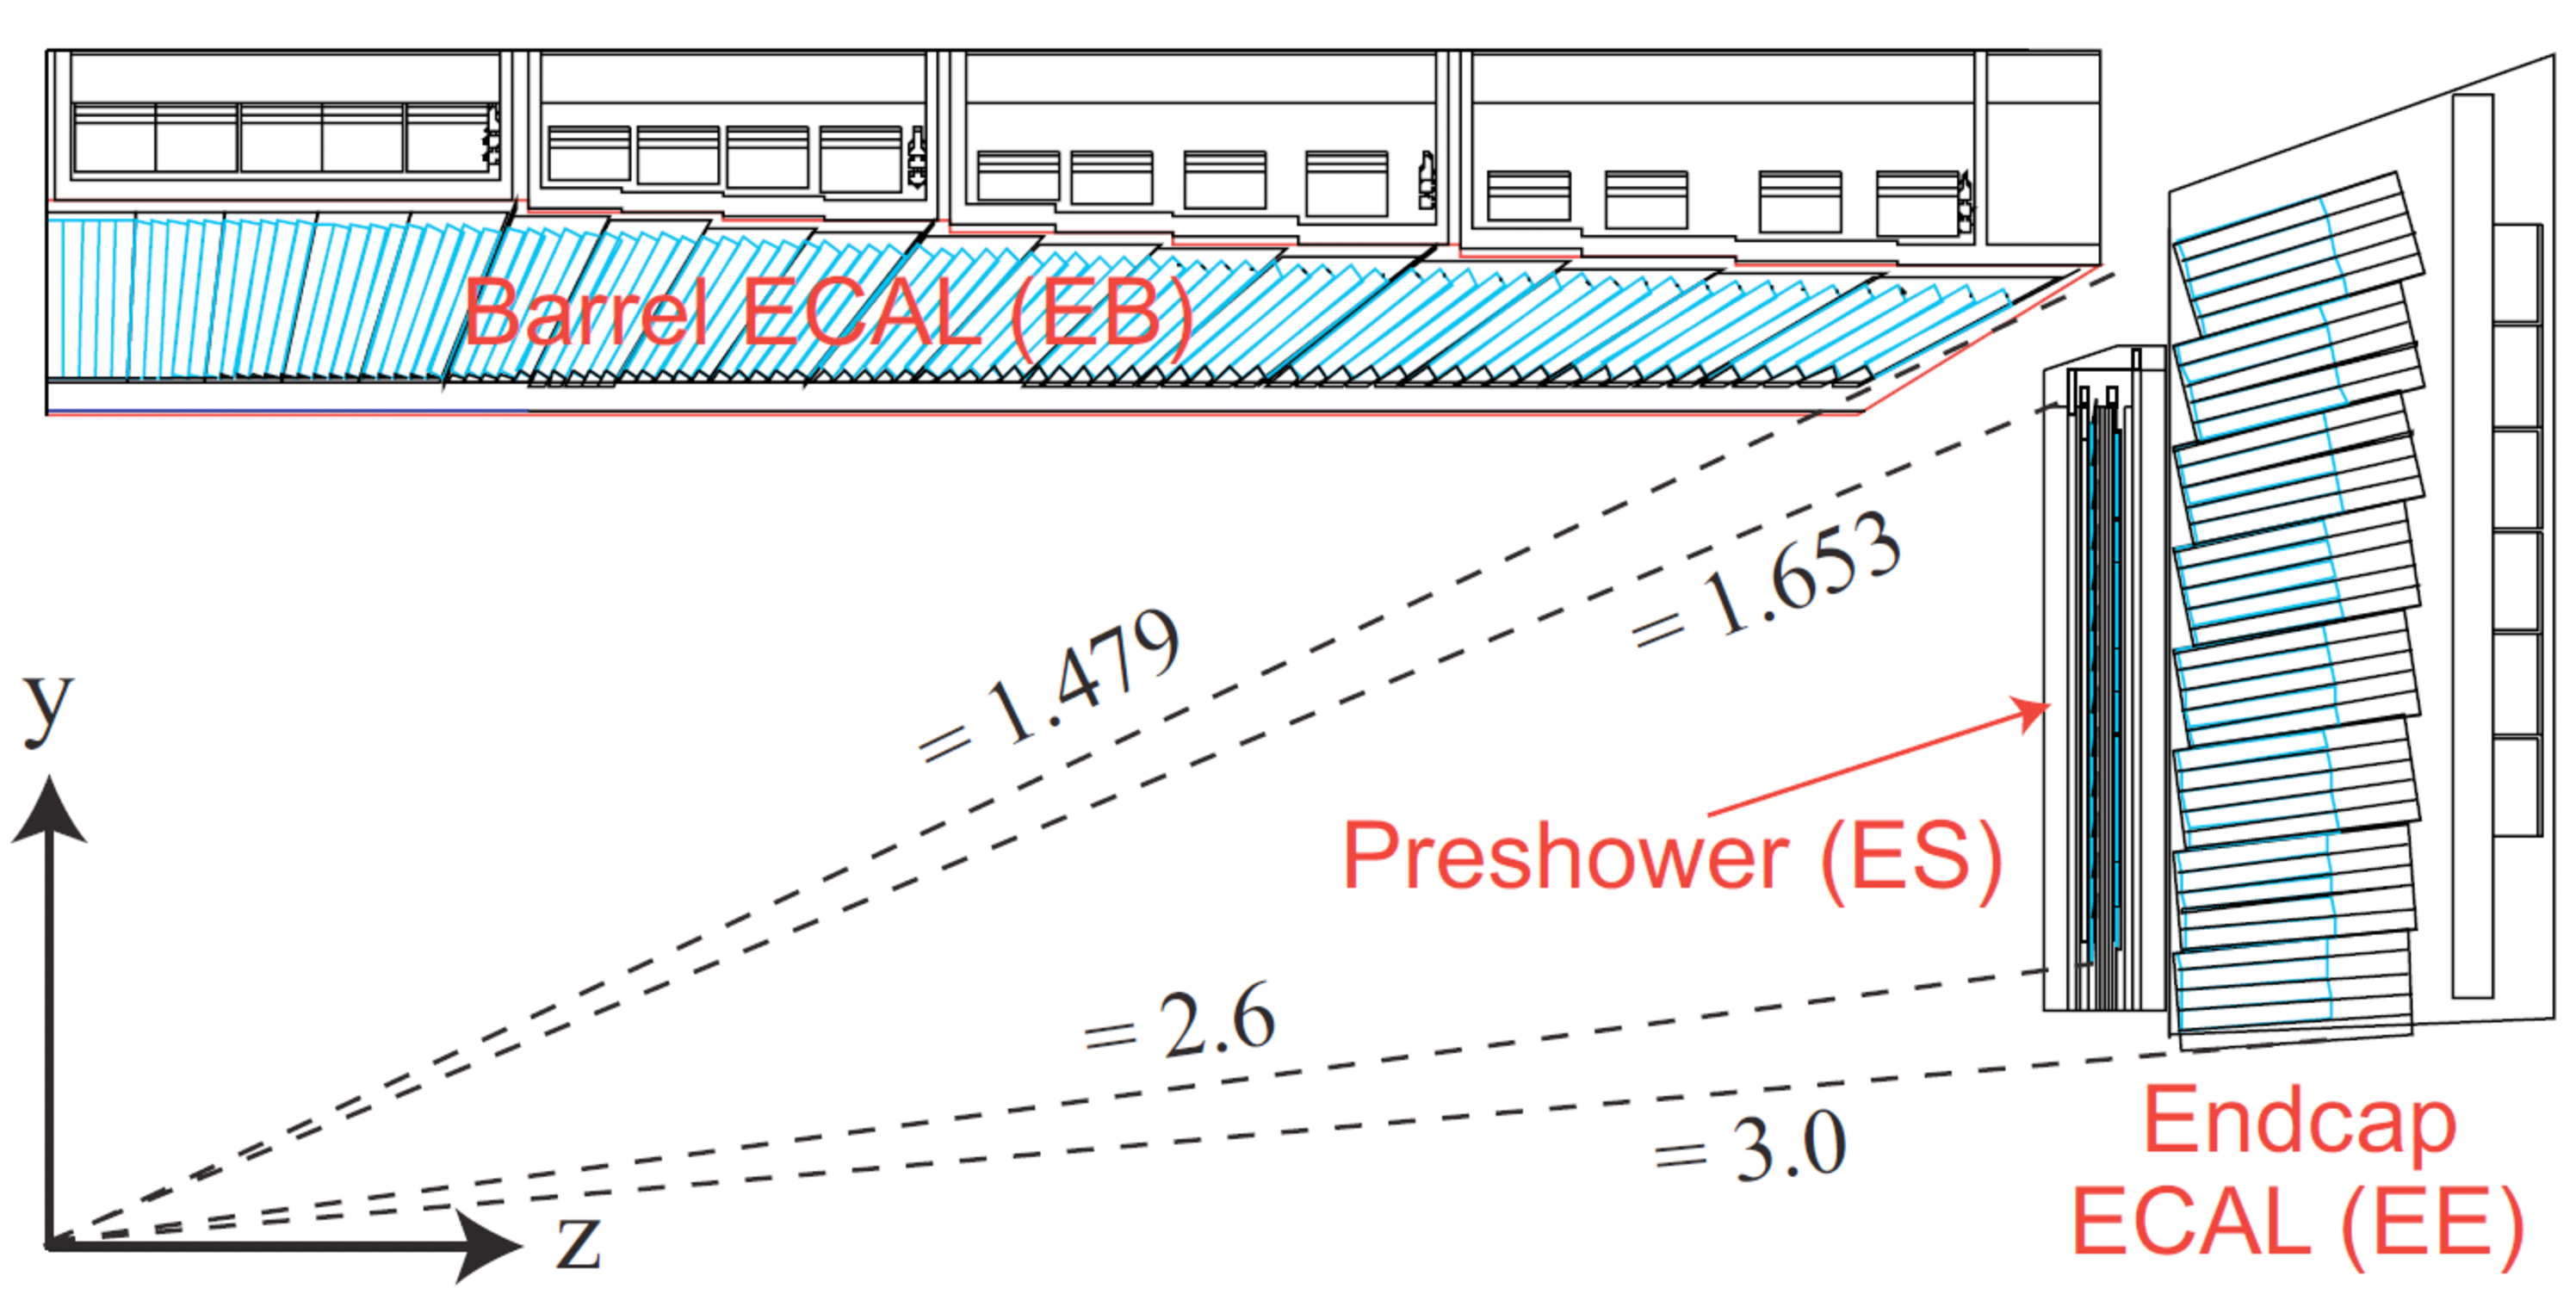
\includegraphics[width=0.9\textwidth]{ecal_rapidity.pdf}
   \caption[text in square brackets]{text in curly brackets}
   \label{fig:cms_ecal}
 \end{center}
\end{figure}


\subsection{HCAL}

\subsection{Solenoid}

\subsection{Muon Chambers}

\subsection{Trigger & Data Acquisition}


% % uncomment the following lines,
% if using chapter-wise bibliography
%
% \bibliographystyle{ndnatbib}
% \bibliography{example}
